
The second test was carried out with the same configurations. Just as before, the method by Brenner et al. (cf. Section \ref{sec: numerical results brenner}) Newton's method did not converge for finer grids. 
Table \ref{tab: l2 errors test 2} shows the error for the pair $k=2$ and $k_{DH}=2$ which is the configuration that converged for the most refinements.

\begin{table}[H]
		\centering
		\pgfplotstabletypeset[
		columns={iterations, l2error, h1error,N},
		every row 0 column 0/.style={set content=init},
		]{\MATwodegTwoTwo}
		\caption{Error for $k=2, k_{DH}=2$ for Test \ref{test sqrt}}
%	\end{subtable}
%	~
%	\begin{subtable}[b]{0.45\textwidth}
%		\centering
%		\pgfplotstabletypeset[columns={iterations, l2error, h1error,N},
%		every row 0 column 0/.style={set content=init},
%		]{\MATwodegThreeThree}
%		\caption{Error for $k=3, k_{DH}=3$}
%	\end{subtable}
%	\caption{Errors }
	\label{tab: l2 errors test 2}
\end{table}
 
Note that Neilan did not give any numerical results for the original method, i.e. without penalty terms, for any test cases with non-smooth solutions. The performance on this test suggest that the non-penalised method is not suitable for irregular solutions. 
% Again the size of the system matrices exceeded memory and therefore the configuration was adjusted for $k=2,3$.

%\begin{figure}[H]
%\centering
%	
\includegraphics[scale =0.45]{../../FEniCS/diagrams/MA2_Neilan_l2.pdf}
%	\caption{$L^2$ errors for Test \ref{test sqrt} }
%	\label{fig: l2 errors test 2}
%\end{figure}
%\begin{figure}[H]
%	\centering
%	
\includegraphics[scale =0.45]{../../FEniCS/diagrams/MA2_Neilan_h1.pdf}
%	\caption{$H^1$ errors for Test \ref{test sqrt} }
%	\label{fig: h1 errors test 2}
%\end{figure}

%\begin{table}[H]
%\centering
%\begin{subtable}[b]{0.45\textwidth}
%	\pgfplotstabletypeset
%	{
%		k $k_{DH}$ {numerical order}
%		2 1 1.55213
%		2 2 1.63088 
%		3 2 1.64644
%		3 3 1.64841
%	}
%	\caption{numerical order in $L2$ norm}
%	\end{subtable}
%	\begin{subtable}[b]{0.45\textwidth}
%	\pgfplotstabletypeset
%	{
%		k $k_{DH}$ {numerical order}
%		2 1 0.465187
%		2 2 0.473759
%		3 2 0.475829
%		3 3  0.495565
%	}
%	\caption{numerical order in $H1$ norm}
%	\end{subtable}
%	\caption{numerical order with jump penalty in test \ref{test smooth}}
%\label{tab: order jump test 2}
%\end{table}

Switching the penalisation of gradient jumps on the method performs better. Its results are shown in Figure \ref{fig: l2 errors test 2 jump} and Table \ref{tab: l2 errors test 2 jump}. The best results were obtained changing the configuration of the Newton solver again: PETSc's trust region method combined with a $LU$ factorisation was chosen. For the $k=2,3$ memory issues occurred, a more memory-friendly configuration such that Newton's method still converges could not be found. % although an extensive parameter research was preformed.

\begin{figure}[H]
	\centering
	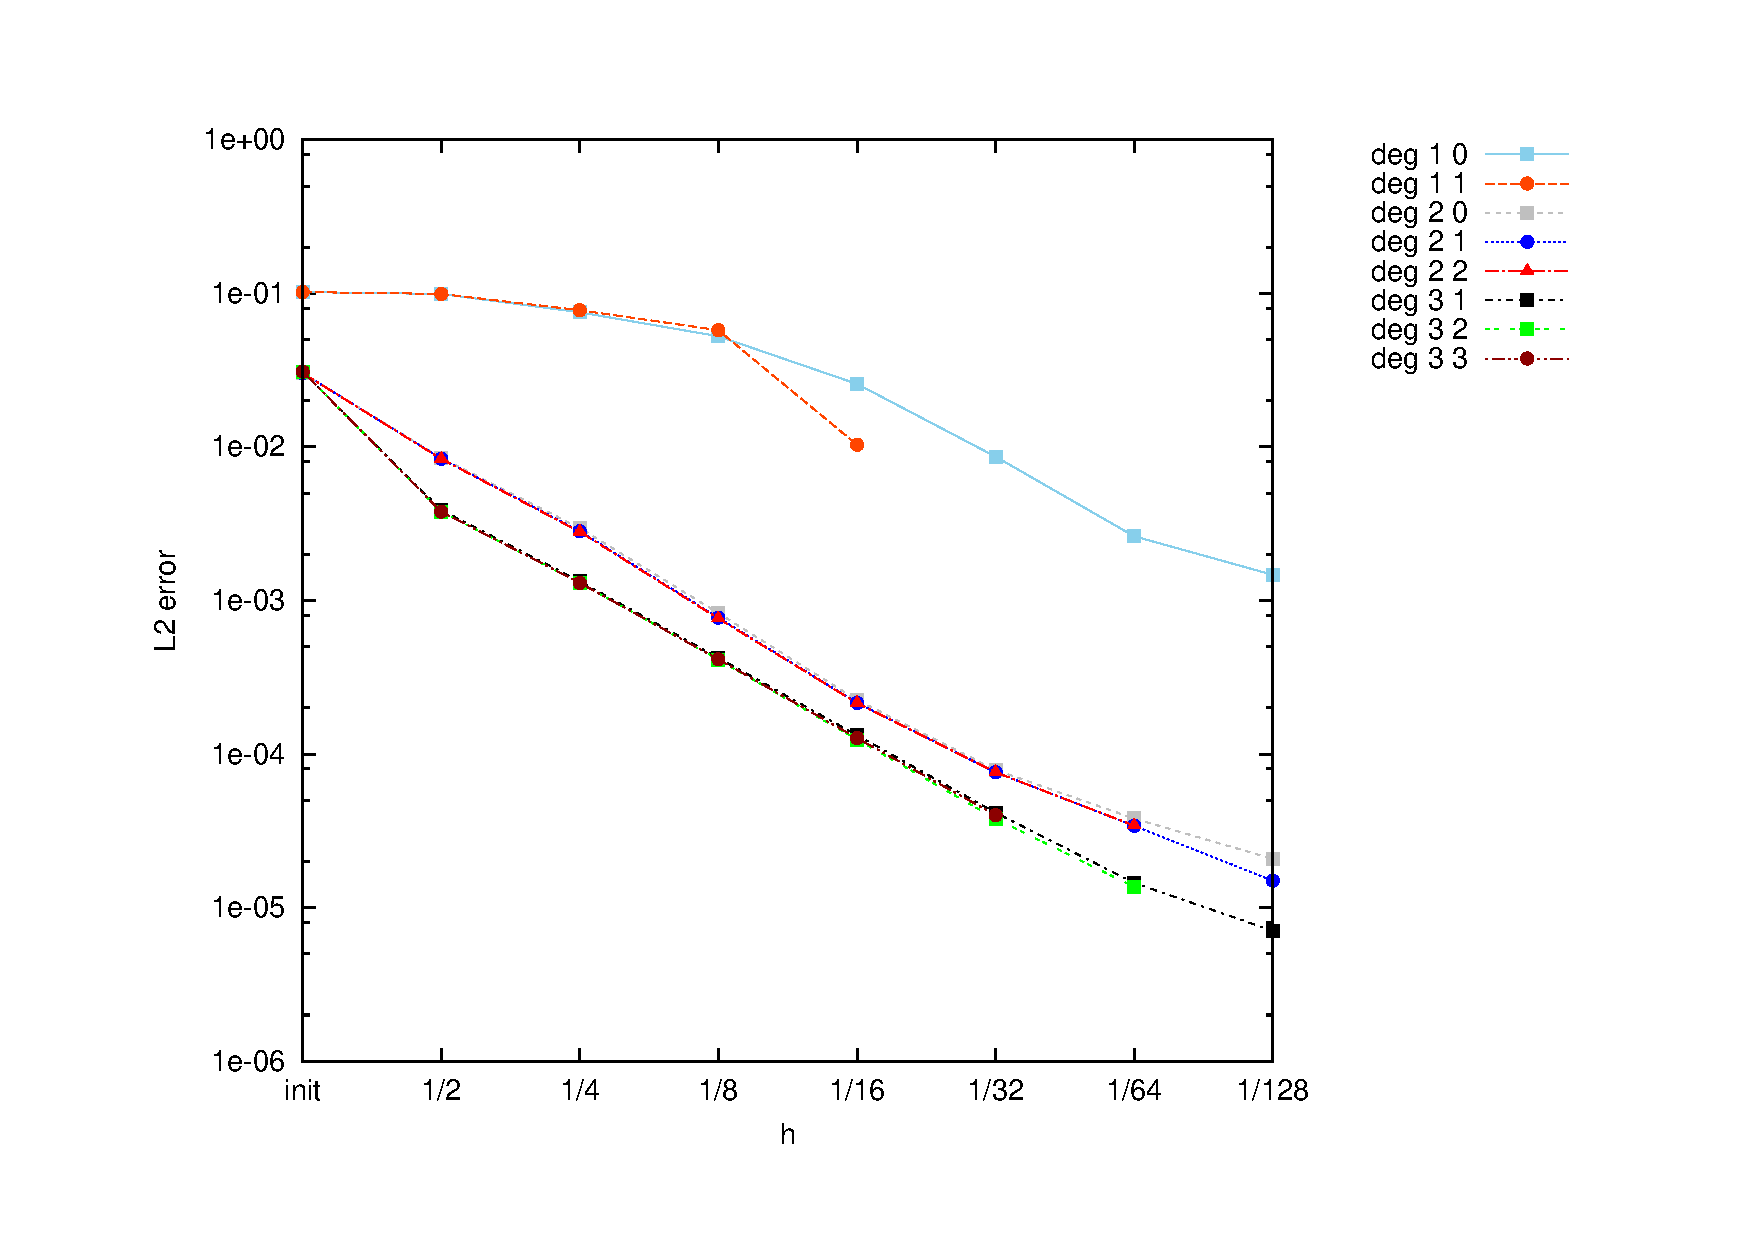
\includegraphics[scale =0.4]{plots/MA2_Neilan_GradJump_l2.pdf}
	\caption{$L^2$ errors for Test \ref{test sqrt}  and additional gradient jump penalty}
	\label{fig: l2 errors test 2 jump}
\end{figure}
\begin{figure}[H]
	\centering
	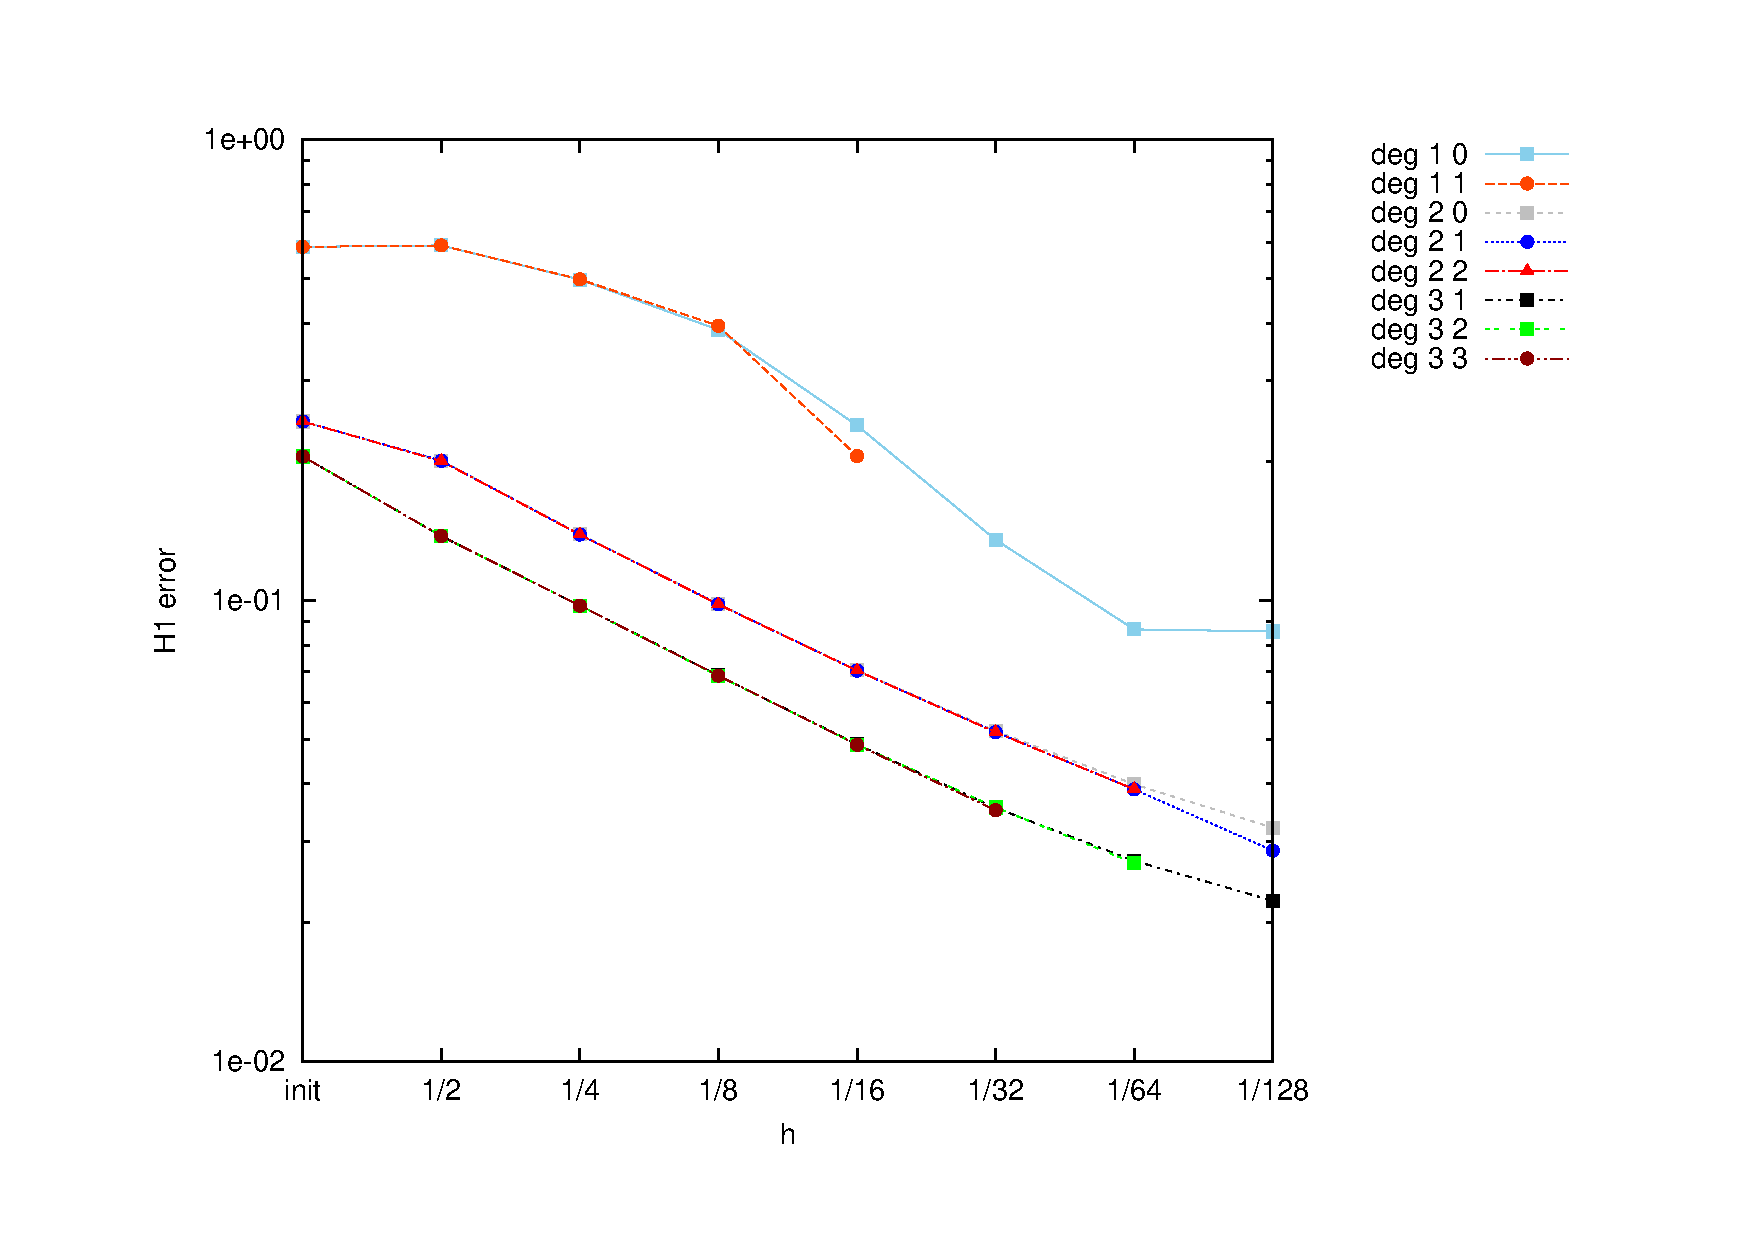
\includegraphics[scale =0.4]{plots/MA2_Neilan_GradJump_h1.pdf}
	\caption{$H^1$ errors for Test \ref{test sqrt}  and additional gradient jump penalty}
	\label{fig: h1 errors test 2 jump}
\end{figure}
\begin{table}[H]
	\begin{subtable}[b]{0.45\textwidth}
		\centering
		\pgfplotstabletypeset[
		columns={iterations, l2error, h1error,N},
		every row 0 column 0/.style={set content=init},
		]{\MATwoJumpdegTwoTwo}
		\caption{Error for $k=2, k_{DH}=2$}
	\end{subtable}
	~
	\begin{subtable}[b]{0.45\textwidth}
		\centering
		\pgfplotstabletypeset[columns={iterations, l2error, h1error,N},
		every row 0 column 0/.style={set content=init},
		every row 6 column 1/.style={set content=-},
		every row 6 column 2/.style={set content=-},
		every row 6 column 3/.style={set content=-},
		]{\MATwoJumpdegThreeThree}
		\caption{Error for $k=3, k_{DH}=3$}
	\end{subtable}
	\caption{Errors for Test \ref{test sqrt} with additional jump penalty}
	\label{tab: l2 errors test 2 jump}
\end{table}

Since the exact solution lacks $H^2$ regularity we do not expect that we benefit from choosing large polynomial degrees. The results also show that the runs with $k=3$ yield only slightly better approximations. The numerical orders given in Table \ref{tab: order jump test 2} confirm this impression. % and the numerical orders for both do not 

\begin{table}[H]
\centering
\begin{subtable}[b]{0.45\textwidth}
	\pgfplotstabletypeset
	{
		k $k_{DH}$ {numerical order}
		1 0 1.08946 
	%	2 0 1.49949
		2 1 1.55213
		2 2 1.63088
		3 2 1.64644
		3 3 1.64841 
	}
	\caption{Numerical order in $L^2$ norm}
	\end{subtable}
	\begin{subtable}[b]{0.45\textwidth}
	\pgfplotstabletypeset
	{
		k $k_{DH}$ {numerical order}
		1 0 0.532518 
	%	2 0 0.445152
		2 1 0.465187
		2 2 0.473759
		3 2 0.475829
		3 3 0.495565
	}
	\caption{Numerical order in $H^1$ norm}
	\end{subtable}
	\caption{Numerical order with jump penalty in test \ref{test singularity}}
\label{tab: order jump test 2}
\end{table}
